
\capitulo{METODOLOGIA}

\iniciocapitulo
A resolução deste trabalho está dividida nas seguintes partes instalação do ambiente, análise e algorítimo.\par

A implementação do sistema se deve primeiramente a configuração do ambiente para o início do desenvolvimento os seguintes passos devem ser tomados para que o ambiente seja reproduzido novamente. Primeiramente deve se instalar o SGBD PostgreSQL, logo em seguida deve se instalar o JAVA 7 em sua maquina, para validar a instalação deve-se executar o seguinte comando "java -version && javac -version" a mensagem descrita na figura XX deve ser mostrada.

\begin{figure}[!htb]
\caption[Versão Java]{Versão Java}
\label{fig:figura2}
\centering
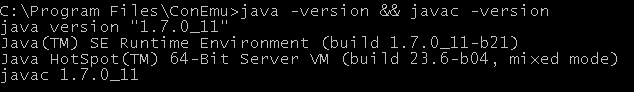
\includegraphics[scale=0.8]{imagens/mensagemJava.png}
\\ \textbf{\footnotesize Fonte: Autor}
\end{figure}


Após a instalação do java deve-se instalar o framework Play! seguindo os passos encontrados no site \cite{play} para validar a instalação do Play! deve se executar o comando "play version" e o \textit{prompt} de comando deve retornar a mensagem conforme mostra a figura figura XX.

\begin{figure}[!htb]
\caption[Versão Framework]{Versão Framework}
\label{fig:figura2}
\centering
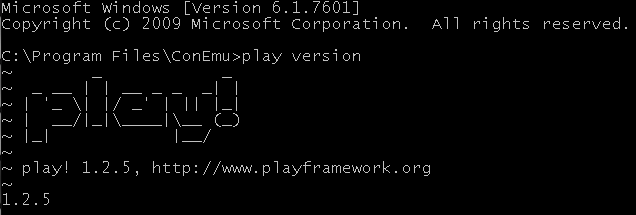
\includegraphics[scale=0.8]{imagens/mensagemPlay.png}
\\ \textbf{\footnotesize Fonte: Autor}
\end{figure}

Uma vez que o ambiente já está configurado devemos inciar um projeto no framework instalado através do comando "play new nomeDoProjeto", a partir dai é possível escolher IDE que será utilizada.

Foi criado um \textit{script} para criação do banco de dados e população inicial das informações como, prédios, salas, turnos, horários, e disciplinas com informações que são necessárias em todo inicio de semestre na instituição de ensino escolhida.

PQ do algoritimo genetico
segundo renand dupas a escolha de algoritimoes geneticos se dá através de uma comparação com outras técnicas e através disso de uma evidenciação das vantagens de sua utilização , logo o algoritimo genetico foi escolhido para este trabalho.

População inicial = --UMA NOVA ABORDAGEM PARA AUMENTAR A DIVERSIDADE.pdf

modelo matematico ----APLICAÇÃO DE MODELO MATEMÁTICO, ABORDAGEM HEURÍSTICA E MÉTODO MISTO NA OTIMIZAÇÃO DA PROGRAMAÇÃO DE HORÁRIO DOS PROFESSORESTURMAS.pdf

restrições do problema e modelo matematico http://www.dcc.ufla.br/infocomp/artigos/v4.3/art08.pdf

Foi realizada uma análise dos requisistos atravez de entrevista com o steakholder, após as entrevistas a modelagem de dados foi realizada de acordo com a demanda do projeto, para o desenvolvimento destes diagramas foi utilizadas a UML (Universal Modeling Language). Os seguintes diagramas foram desenhados, diagrama de caso de uso, diagrama de classe e diagrama de entidade relacionamento. Foram escolhidos os seguintes diagramas para que o sistema tenha uma documentação minima tendo em vista que o foco do trabalho é a resolução do problema de timetable através da utilização do algoritimo genetico.

Por se tratar de um sistema complexo, antes de iniciar a implementação do sistema
fez-se necessário a sua modelagem. Segundo Elmasri & Navathe (2005) as metodologias
de modelagem de dados de objetos como UML (Universal Modeling Language –
Linguagem de Modelagem Universal) estão se tornando cada vez mais populares no
projeto e engenharia de software. Essas metodologias vão além do projeto de um banco de
dados, especificando o projeto detalhado dos módulos de software e suas interações,
utilizando vários tipos de diagramas.\par

\secao{Ferramentas Utilizadas}

Este trabalho conta com a utilização de tecnologias proprias para o desenvolvimento de sistemas web, foram utilizadas as seguintes ferramentas: Para SGBD foi o utilizado PostgreSQL; No back-end foi utilizado Java e o \textit{framework Play!}; No front-end as tecnologias utilizadas foram HTML, CSS, JavaScript e \textit{framework AngularJS} e a IDE utilizada \textit{Eclipse}.\par



\subsecao{Sistema de Gerenciamento de Banco de Dados}

O SGBD escolhido foi o PostgreSQL pelo fato de ser uma ferramenta open-source e que trabalha perfeitamente com o framework escolhido Play!, uma vez que utilizado em projetos anteriores não foram apresentados conflitos entre o framework e o SGBD. A seguir pode ser notar que é uma ferramenta robusta e que tem visão no mercado internacional.\par

O PostgreSQL é um poderoso sistema gerenciador de banco de dados objeto-relacional de código aberto.  Tem mais de 15 anos de desenvolvimento ativo e uma arquitetura que comprovadamente ganhou forte reputação de confiabilidade, integridade de dados e conformidade a padrões.  Roda em todos os grandes sistemas operacionais. É totalmente compatível com ACID, tem suporte completo a chaves estrangeiras, junções (JOINs), visões, gatilhos e procedimentos armazenados (em múltiplas linguagens).  Inclui a maior parte dos tipos de dados do ISO SQL:1999, incluindo INTEGER, NUMERIC, BOOLEAN, CHAR, VARCHAR, DATE, INTERVAL, e TIMESTAMP.  Suporta também o armazenamento de objetos binários, incluindo figuras, sons ou vídeos.  Possui interfaces nativas de programação para C/C++, Java, .Net, Perl, Python, Ruby, Tcl, ODBC, entre outros, e uma excepcional documentação.\cite{postgresql}



Para a resolução do problema de timetable foi escolhido o algoritimo genetico, a escolha do algoritimo foi devida a grande utilização do mesmo para resolução de problemas do tipo NP-dificil que foram encontrados na literatura.
\par




\subsecao{Ferramentas Back-end}

Foi escolhida uma linguagem de programação Java por ser orientada a objeto. Tambem foi escolhido o \textit{Play! framework}, para que o desenvolvimento aconteça de forma mais rápida, fácil e eficiente.\par

%Java
Java foi criada pela Sun Microsystems para desenvolver inovações tecnológicas em 1992, time liderado por James Gosling. O Java utiliza do conceito de máquina virtual, onde existe, entre o sistema operacional e a aplicação, uma camada extra responsável por \"traduzir\" - mas não apenas isso - o que sua aplicação deseja fazer para as respectivas chamadas do sistema operacional, onde ela está rodando no momento. Sua aplicação roda sem nenhum envolvimento com o sistema operacional, sempre conversando apenas com a JVM - Java Virtual Machine \cite{caelum}.\par

Em 2009 a Oracle comprou a Sun, fortalecendo a marca. A Oracle sempre foi, junto com a IBM, uma das empresas que mais investiram e fizeram negócios através do uso da plataforma Java. Em 2011 surge a versão Java 7 com algumas pequenas mudanças na linguagem \cite{caelum}.\par

%-----Play! Framework

The Play! É um moderno framework MVC de alta produtividade, que utiliza Java e Scala para o desenvolvimento web, open-source , utiliza templates, hibernate e JUnit  em sua arquitetura. Existe duas versões do framework Play! 1 e Play2! este trabalho utiliza a versão 1 do framework\cite{playframework}.\par


\subsecao{Ferramentas Front-end}

As ferramentes de Front-end descritas abaixo, foram escolhidas devida a gande utilização na web grande parte dos sites contem HTML, CSS ou JavaScript em algum trexo de seu código, foi escolhido tambem o framework AngularJS para que o desenvolvimento ocorra de maneira agil e mais rapida.\par

%HTML
HTML que é defindo por (\textit{HyperText Markup Language}) ou linguagem de marcação, é uma linguagem que é utilizada no desenvolvimento de paginas web \cite{html}.\par

%css
Cascading Style Sheets (CSS) é uma tecnologia utilizada para adicionar estilos como cores, fontes, espaçamentos em documentos escritos em uma linguagem de marcação como exemplo o HTML \cite{css}.\par

%JAVASCRIPT

JavaScript é uma linguagem de script utilizada no desenvolvimento de paginas na web, atualmente é a principal linguagem para programação client-side em navegadores web. Todas as paginas de HTML modernas estão usando JavaScript para adicionar funcionalidades e para se comunicar com os webServers\cite{javascript}.\par

Angularjs é um \textit{framework JavaScript} construido e mantido pelo grupo de engenheiros do Google, ele usa o HTML como uma \textit{template engine}, tudo isso no intuito de fornecer uma solução completa para o cliente-side de sua aplicação. Além disso tem total compatibilidade com as bibliotecas javascript mais utilizadas, como jQuery. É um novo conceito para desenvolvimento de web apps client-site.\cite{angularjs}\par

\subsecao{IDE}

O Eclipse é uma IDE (\textit{integrated development environment}). Diferente de uma RAD(\textit{Rapid Application Development}), onde o objetivo é desenvolver o mais rápido possível através do arrastar-e-soltar do mouse, onde montanhas de código são gerados em background, uma IDE te auxilia no desenvolvimento, evitando se intrometer e fazer muita mágica \cite{caelum}.\par

O Eclipse é a IDE líder de mercado. Formada por um consórcio liderado pela IBM, possui seu código livre. A última versão é a 4.3, mas com qualquer versão posterior a do 3.1 você terá suporte ao Java 5, 6 e 7 \cite{caelum}.\par

Está IDE foi escolhida devido ao grande reconhecimento mundial, por sua eficiencia ao se trabalhar com a linguagem de programação Java, por ser open-source e pela existencia de varias ferramentas criadas pela comunidade, para o auxilio no desenvolvimento de softwares.\par